\chapter{Discussion 5: Conductors}

\section{Properties of Conductors}
\begin{enumerate}
		\item $E = 0$ inside conductors. 
				\begin{itemize}
						\item If the electric field were not zero then the charges would continue moving until
								the electric field settled down.
						\item The charge density is 0 inside conductors.
				\end{itemize}
		\item $\rho = 0$ inside conductors (charge density is 0 inside a conductor) {\text{red}{why is this true?}}
		\item All net charge of a conductor exists on its surface.
				\begin{itemize}
						\item This follows directly from the previous part -- there's nowhere else for the charges
								to go. 
				\end{itemize}
		\item A conductor is an equipotential
				\begin{itemize}
						\item If the conductor were not an equipotential then $-\grad V = E \neq 0$, violating the 
						first property
				\end{itemize}
		\item The electric field $\mathbf E$ is perpendicular to the surface with magnitude 
				$E = \frac{\sigma}{\epsilon_0}$
				\begin{itemize}
						\item From the fact that conductors are an equipotential, so the gradient must be 
								perpendicular. The magnitude follows from calculating the electric field for a 
								Gaussian pillbox. 
				\end{itemize}
\end{enumerate}

\section{Response to Charge}

Conductors will respond to the presence of charge by attempting to cancel the electric field generated by the 
outside charge. If necessary, the conductor will exhibit polarization (when charges inside the conductor are moved
around, causing a slight uneven distribution in the charge. 

\begin{example}
		Find $\sigma_a, \sigma_b, \sigma_R$ given the following diagram: 

		\begin{center}
				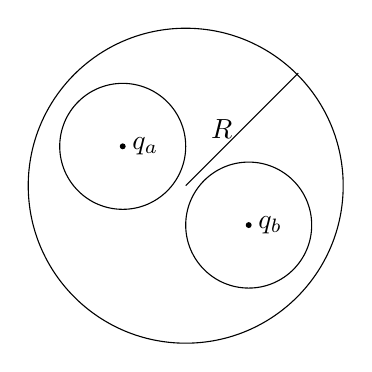
\begin{tikzpicture}
						\draw (0, 0) circle (2cm); 
						\draw (-0.8, 0.5) circle (0.8cm);
						\draw (0.8, -0.5) circle (0.8cm);
						\filldraw(-0.8, 0.5) circle (0.03cm) node[right] {$q_a$};
						\filldraw(0.8, -0.5) circle (0.03cm) node[right] {$q_b$};
						\draw (0, 0) -- node[midway, above, left] {$R$}   (1.43, 1.43); 
				\end{tikzpicture}
		\end{center}
\end{example}



